\documentclass[12pt]{article}
\usepackage[centering]{geometry}
\usepackage{graphicx}

\begin{document}

We start off by running the model for $i = 1$ critical island size to compare to previous results. Amar and Family did some scaling analysis for the high $R = D/F$ regime, so we focus our model runs on this regime. In their papar, Amar and Family presented results for $R = 8$ and $R = 9$ for critical island size $i = 1$. We managed to get a lot of model output for $R = 8$, but it took quite a bit of computing time to get it all. Unfortunately, it seems the model I wrote is horribly inefficient for some reason, and I have just not produced enough $R = 9$ output to really smooth out the results.


\begin{figure}
\begin{center}
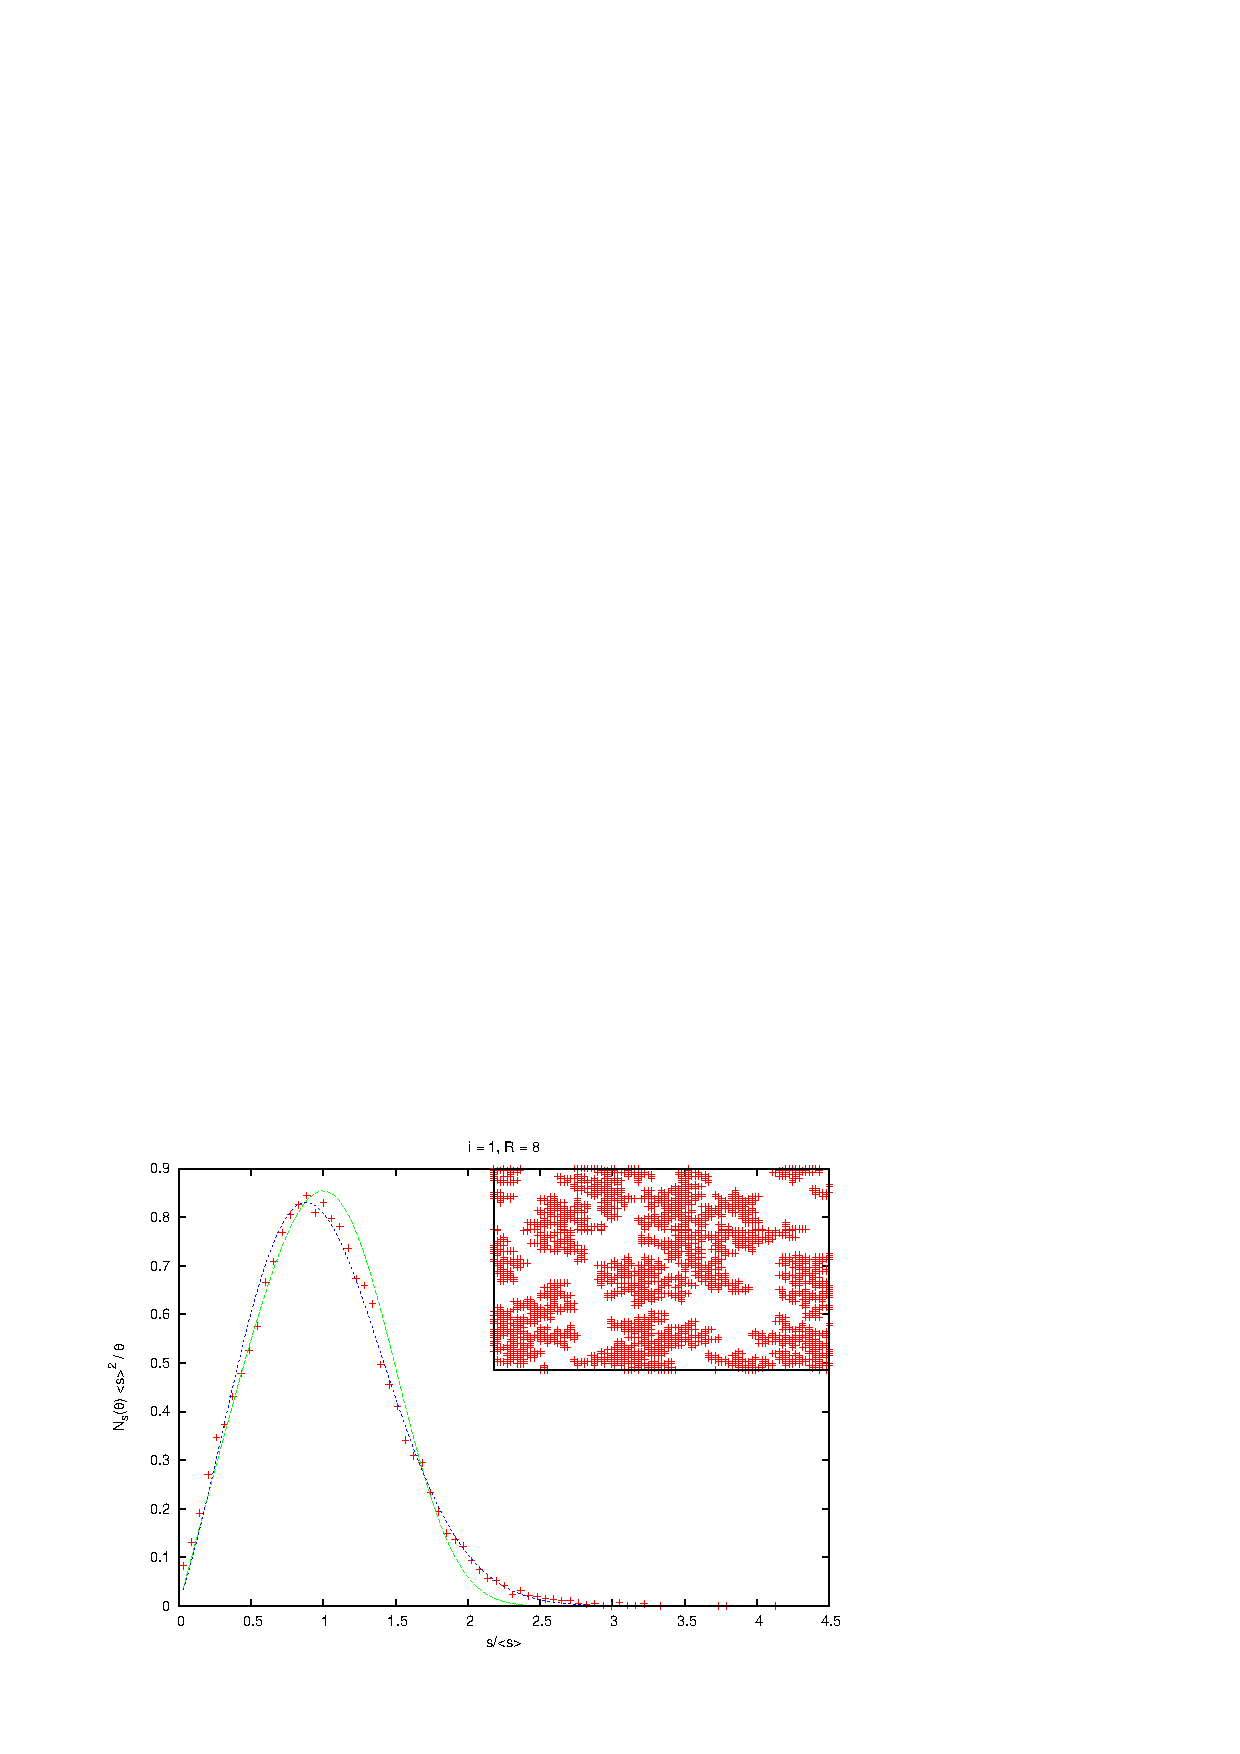
\includegraphics[width=0.80\linewidth]{../../sizes/i1r8.pdf} \\
\end{center}
\caption{Critical island size $i = 1$ scaling distributions for $R = 10^8$.}
\end{figure}

\begin{figure}
\begin{center}
\includegraphics[width=0.80\linewidth]{../../sizes/i1r9.pdf}
\end{center}
\caption{Critical island size $i = 1$ scaling distributions for $R = 10^9$.}
\end{figure}

Next, we set out to reproduce the results of Amar and Family for critical island size $i = 3$. This corresponds to an extra activation energy for monomers with between one and two neighbors to break away from their neighbors and diffuse. Our definition of the activation energy $E_1$ is similar to that discussed in the Family paper. $E_1$ is the activation energy for diffusion of monomers with $1$ neighbor, which corresponding relative diffusion rate $\tau_1 = D_1/D = e^{(E_0 - E_1)/kT}$, where $E_0$ is the activation energy for free monomers, which is taken to be zero in this implementation.

We have ran the model for $R = 10^9$ and $R = 10^{10}$ with $E_1 = 0.30$, however there is not nearly enough model output to even make a readable plot for $R = 10^{10}$. These runs take entirely too much time. I think any effort to look at diffusion this high is going to take a substantial rewrite of the code, probably by someone more intelligent than I am as I could not see any way to drastically speed it up.

What we have for the high-ish $R$ regime may be enough to say something about the gaussian versus the Family scale functions. For $i = 1$ the gaussian certainly seems to fit the output better, for the clear case of $R = 10^8$ anyways. The $i = 3$ gaussian also seems to be a better fit than the $i = 3$ Family curve, although neither of them seem to fit all that well. We may really benefit from higher $R$, but with the current code it could just not happen on reasonable time scales.

\begin{figure}
\begin{center}
\includegraphics[width=0.80\linewidth]{../../sizes/i3r9.pdf}
\caption{Critical island size $i = 3$ scaling distributions for $R = 10^9$, with activation energy for single neighbor monomers $E_1 = 0.3$.}
\end{center}
\end{figure}

\end{document}
